To run Wireshark together with the custom Lua script for dissecting the protocol defined in this thesis run
\begin{itemize}
  \item \texttt{wireshark -X lua\_script:wireshark/dissector.lua}
\end{itemize}
while in the root directory of the project. However, this dissector only works if the application is using the default port \texttt{4040}. Below are some captured examples.
\begin{figure}[ht!]
  \centering
  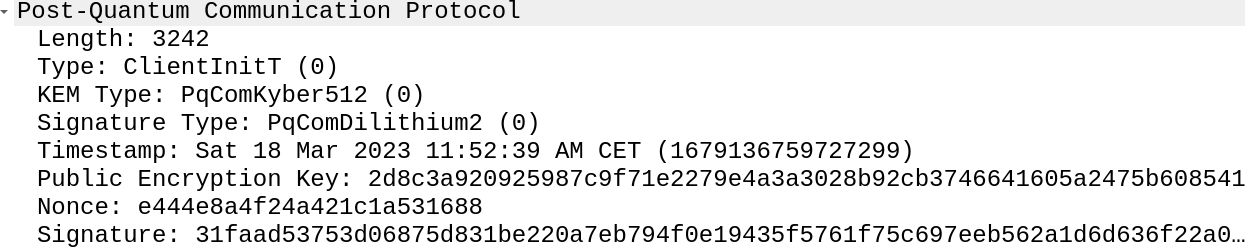
\includegraphics[width=\textwidth]{pictures/clientinit.png}
  \caption{Captured client init}
  \label{img:cap_clientinit}
\end{figure}

\begin{figure}[ht!]
  \centering
  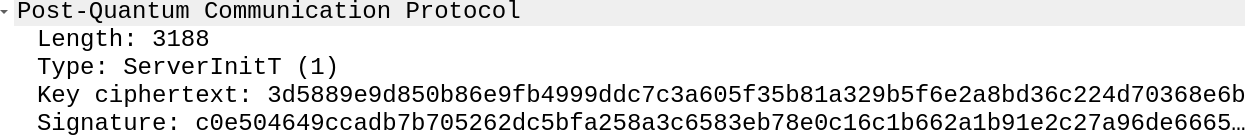
\includegraphics[width=\textwidth]{pictures/serverinit.png}
  \caption{Captured server init}
  \label{img:cap_serverinit}
\end{figure}

\begin{figure}[ht!]
  \centering
  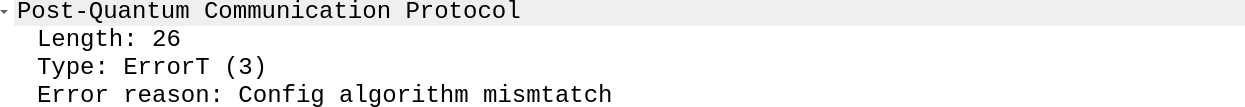
\includegraphics[width=\textwidth]{pictures/error.png}
  \caption{Captured error}
  \label{img:cap_error}
\end{figure}

\begin{figure}[ht!]
  \centering
  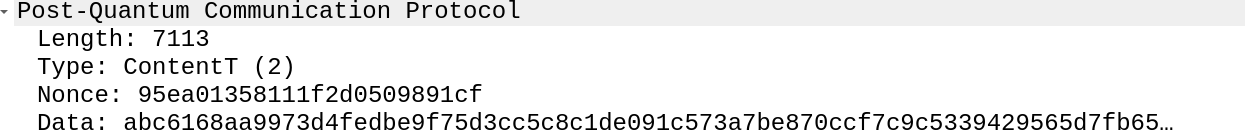
\includegraphics[width=\textwidth]{pictures/data.png}
  \caption{Captured data}
  \label{img:cap_data}
\end{figure}
